\section{Functions}
\textbf{Definition} A function is a correspondence between input numbers(x-values) and output numbers(y-values) such that each input number is paired with exactly one output number. \\
A non-mathematical example of a function is a vending machine. The input is the money(x-values) you put in and the output is the item you get(y-values). You can't put in the same amount of money and get two different items. \\

Functions can be described with an equation.
\\
\textbf{Example}. $y = x^2 + 1$, which can also be written as $f(x) = x^2 + 1$. \\
\vspace{4pt}

What is $f(2)$ ? $ f(5) ?$ \\
\vspace{4pt}

In mathematics, the notation "f(x)" is commonly used to represent a function. In this notation, "f" is the name of the function, and "x" is the input or independent variable. When you write "f(x)," you are essentially saying "the value of the function f when the input is x."

The function itself is a rule or relationship that assigns a unique output (often denoted as "y") for each input value "x." So, when you evaluate "f(x)," you are finding the corresponding output value for the given input.

Here's a simple example to illustrate this:

Let's say you have a function defined as:
f(x) = 2x + 3

If you want to find the value of the function when x is 4, you would write it as:
$f(4) = 2 \cdot 4 + 3 = 8 + 3 = 11$

So, in this case, f(4) refers to the y-value or the output of the function when x is 4, and it equals 11. The notation "f(x)" is just a way to represent this relationship between inputs (x-values) and outputs (y-values) in a concise and standardized manner.

When we write $f(2)$, we are asking what is the value of the function when $x = 2$. \\
So we take $2$ and plug it in for $x$ in the equation. \\

$$f(2) = 2^2 + 1 = 5$$
$$f(5) = 5^2 + 1 = 26$$ \\

Similarly, we can ask what is $f(a + 3)$
$$ f(a + 3) = (a+3)^2 + 1 = a^2 + 6a + 10 $$
\vspace{4pt}

We can also describe a function with a graph. \\
\textbf{Example}. The graph if $y = g(x)$ is shown below
\begin{align*}
	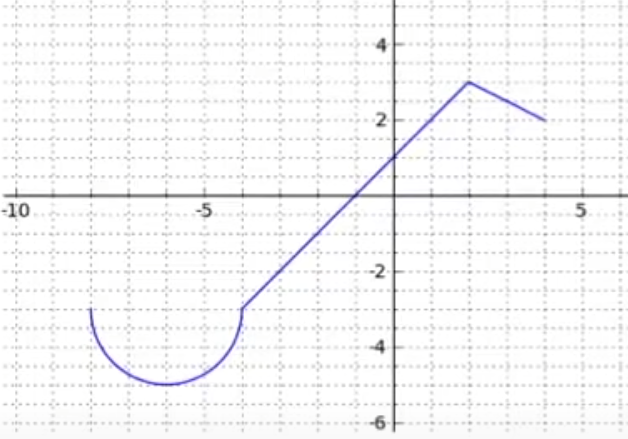
\includegraphics{algebra-pre-calculus/functions/graph1.png}
\end{align*}
\vspace{1pt}
What is $g(2)$ ? $ g(5) ?$ \\

First let's establish that $ y = g(x) $ so they are essentially mean the same thing. \\
In $g(2)$, $2$ corresponds to the $x$-value and we will use the graph to find corresponding $y$-value. \\
Since we know that we have to look for the $x$-value of $2$, we can look at the graph and find the point where $x = 2$. \\
Then we can look at the $y$-value of that point and that will be $3$. \\
Therefore, $g(2) = 3$. \\
Now when we look at $g(5)$, we can use the same method. However, we run into an issue that when we look at the x-value of $5$, we see that there is no point on the graph that has that x-value. \\
Therefore, $g(5)$ is undefined. \\
The question of what x-values and y-values makes sense to a function leads to the \textbf{domain} and \textbf{range} for a function. \\

\subsection{Domain and Range of a Function}
\textbf{Domain}: The domain of a function is the set of all possible x-values. \\
\textbf{Range}: The range of a function is the set of all possible y-values. \\

Let's examine the graph again and determine its range and domain. To find the domain of a function we have to look at the x-values that corresponds a point on the graph. \\
\begin{align*}
	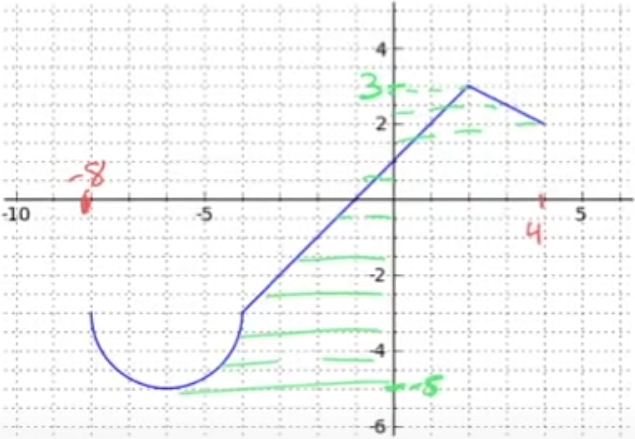
\includegraphics{algebra-pre-calculus/functions/graph2.png}
\end{align*}

We can see that the \textbf{domain} is $-8 \le x \le 4$. \\
Or as an interval notation, $[-8, 4]$. \\

To find the range of a function we have to look at the y-values that corresponds a point on the graph. \\
\textbf{range} is $-5 \le y \le 3$. \\
Or as an interval notation, $[-5, 3]$. \\

\subsection{Domain and Range of a Function as an Equation}
\textbf{Example}. Find the domain of these functions. \\
$\displaystyle A. \ g(x) = \frac{x}{x^2 - 4x + 3}$ \\
$\displaystyle B. \ f(x) = \sqrt{3-2x}$ \\
To find the domain of a function we have to consider algebraic restrictions. We can go ahead and question what values make sense to plug in for $x$. \\
Therefore,
\begin{itemize}
	\item 1. Exclude x-values that make the denominator 0.
	\item 2. Exclude x-values that make the radicand(number under the radical) negative. Since we cannot take the square root of a negative number.
\end{itemize}

What we have to do in the first function is this:
\begin{align*}
	x^2-4x+3 & \neq 0 \quad \text{Since the denominator cannot be 0} \\
\end{align*}

In other words we can solve the equation to be equal to 0 and exclude its solutions
\begin{align*}
	x^2-4x+3   & = 0 \quad \text{Factorise the quadratic} \\
	(x-3)(x-1) & = 0                                      \\
	x          & = 3, 1                                   \\
\end{align*}
Therefore we need to exclude $x=3$ and $x=1$ from the domain. \\

We can represent the domain as an interval notation. \\
\textbf{Domain} is $(-\infty, 1) \cup (1, 3) \cup (3, \infty)$. \\
Meaning that the domain is all real numbers except $1$ and $3$. \\

Now let's look at the second function.

Since we cannot take the square root of a negative number, we have to make sure that the radicand is not negative. \\

Therefore, we exclude the numbers:
$$ 3-2x < 0$$

Similarly we can include everyone number that makes the radicand positive(bigger than zero). \\
$$ 3-2x \ge 0$$
$$ 3 \ge 2x$$
$$ \frac{3}{2} \ge x$$

Therefore, the domain is $(-\infty, \frac{3}{2}]$.
Notice that we used a square bracket instead of a round bracket. This is because we can include the number $\frac{3}{2}$ in the domain. \\

\subsection{Function as a fractional equation with radicals}

\textbf{Example}. $\displaystyle h(x)=\frac{\sqrt{3-2x}}{x^2-4x+3}$ \\

So we have to consider the same restrictions as before. \\

\begin{align*}
	x^2-4x+3 &\neq 0 \quad \text{Since the denominator cannot be 0} \\
	3-2x &\ge 0 \quad \text{Since we cannot take the square root of a negative number} \\
\end{align*}

We've already solved the first condition which was $x\neq3$ and $x\neq1$. \\
The second condition is $x\le\frac{3}{2}$. \\

Therefore our domain is $(-\infty, 1) \cup (1, \frac{3}{2}]$.

\subsection{Increasing and Decreasing Functions}

\textbf{Example.} Which function is Increasing and which is Decreasing?

\begin{align*}
	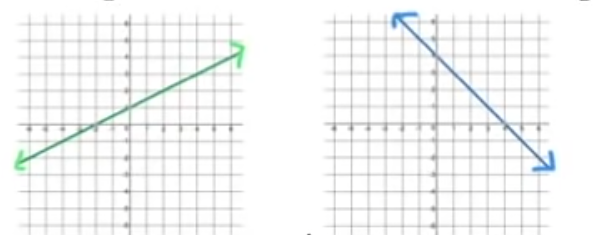
\includegraphics{algebra-pre-calculus/functions/graph3.png}
\end{align*}

As seen the first function is increasing and the second function is decreasing. 

This can be written more formaly as: \\
$ x_1 < x_2 \Rightarrow f(x_1) < f(x_2) $ \\
$x_1$ and $x_2$ are two arbitrary x-values. \\
This means that the y-values are increasing as the x-values are increasing. \\

In the decreasing function, the y-values are decreasing as the x-values are increasing. 
$ x_1 < x_2 \Rightarrow f(x_1) > f(x_2) $ \\

\textbf{Example.} On what intervals is the function graphed below increasing? Decreasing? 
\begin{align*}
	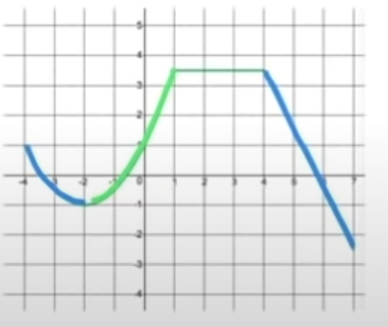
\includegraphics{algebra-pre-calculus/functions/graph4.png}
\end{align*}

We are going to solve this in terms of the x-values. Simply because the y-values can be same for different parts of the graph but the x-values are unique.
\textbf{Decreasing}: $-4\le x<-2, \quad 4<x\le7 $ \\
\textbf{Increasing}: $-2< x<1$ \\
As intervals: $[-4, -2) \cup (4,7), (-2, 1)$ \\

\subsection{Maximums and Minimums on Graphs}
\textbf{Definition.} An absolute maximum of a function, also known as a global maximum, is the highest value that the function can attain over its entire domain. In other words, it is the largest output (or y-value) that the function can produce for any input (or x-value) within its defined domain. \\
In other words a function f(x) has an absolute maximum at $x = c$ if $f(c) \ge f(x)$ for all $x$ in the domain of $f$. \\
The y-value f(c) is called the absolute maximum value of $f$. \\
and the point $(c, f(c))$ is called the absolute maximum point of $f$. \\

\begin{align*}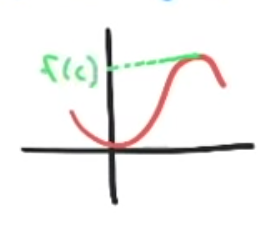
\includegraphics{algebra-pre-calculus/functions/graph5.png}\end{align*}
Here we can see that essentially the absolute maximum is the highest point on the graph. \\
And the absolute value point would be the point where it achieves the absolute maximum. \\
A function can have multiple absolute maximum points(multiple points referencing to the absolute maximum of the function), however it can only have one absolute maximum value. \\

\textbf{Definition}. The absolute minimum of a function, also known as a global minimum, is the lowest value that the function can attain over its entire domain. In other words, it is the smallest output (or y-value) that the function can produce for any input (or x-value) within its defined domain. \\
The absolute minimum of a function $f(x)$ is the smallest value of $f(x)$ over its entire domain. \\
In other words a function f(x) has an absolute minimum at $x = c$ if $f(c) \le f(x)$ for all $x$ in the domain of $f$. \\
The y-value f(c) is called the absolute minimum value of $f$. \\
and the point $(c, f(c))$ is called the absolute minimum point of $f$. \\

\begin{align*}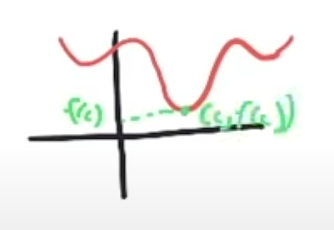
\includegraphics{algebra-pre-calculus/functions/graph6.png}\end{align*}
Here we can see that essentially the absolute minimum is the lowest point on the graph. \\
And the absolute value point would be the point where it achieves the absolute minimum. \\
A function can have multiple absolute minimum points(multiple points referencing to the absolute minimum of the function), however it can only have one absolute minimum value. \\
\newpage
\subsection{Local Maximums and Minimums}
\textbf{Definition.} A local maximum of a function is a point on the graph where the y-value is greater than or equal to all the y-values of points in the nearby region. \\
A function f(x) has a local maximum at $x = c$ if $f(c) \ge f(x)$ for all $x$ in some open interval around $c$. \\

In other words, the way we identify local maximums is by looking at the graph and seeing if there is a point where an interval around that point exists such that all function values within that interval are less than or equal to the function value at that specific point. If this condition is met, we can conclude that the function has a local maximum at that point.

A local minimum of a function is a point on the graph where the y-value is less than or equal to all the y-values of points in the nearby region. \\
A function f(x) has a local minimum at $x = c$ if $f(c) \le f(x)$ for all $x$ in some open interval around $c$. \\
In other words, the way we identify local minimums is by looking at the graph and seeing if there is a point where an interval around that point exists such that all function values within that interval are greater than or equal to the function value at that specific point. If this condition is met, we can conclude that the function has a local minimum at that point. \\

\textbf{Definition}. Local maximum and minimum points are also called relative maximum and minimum points. \\
\textbf{Definition}. A point where a function changes from increasing to decreasing or decreasing to increasing is called a turning point. \\

\newpage
\begin{figure}
	\centering
	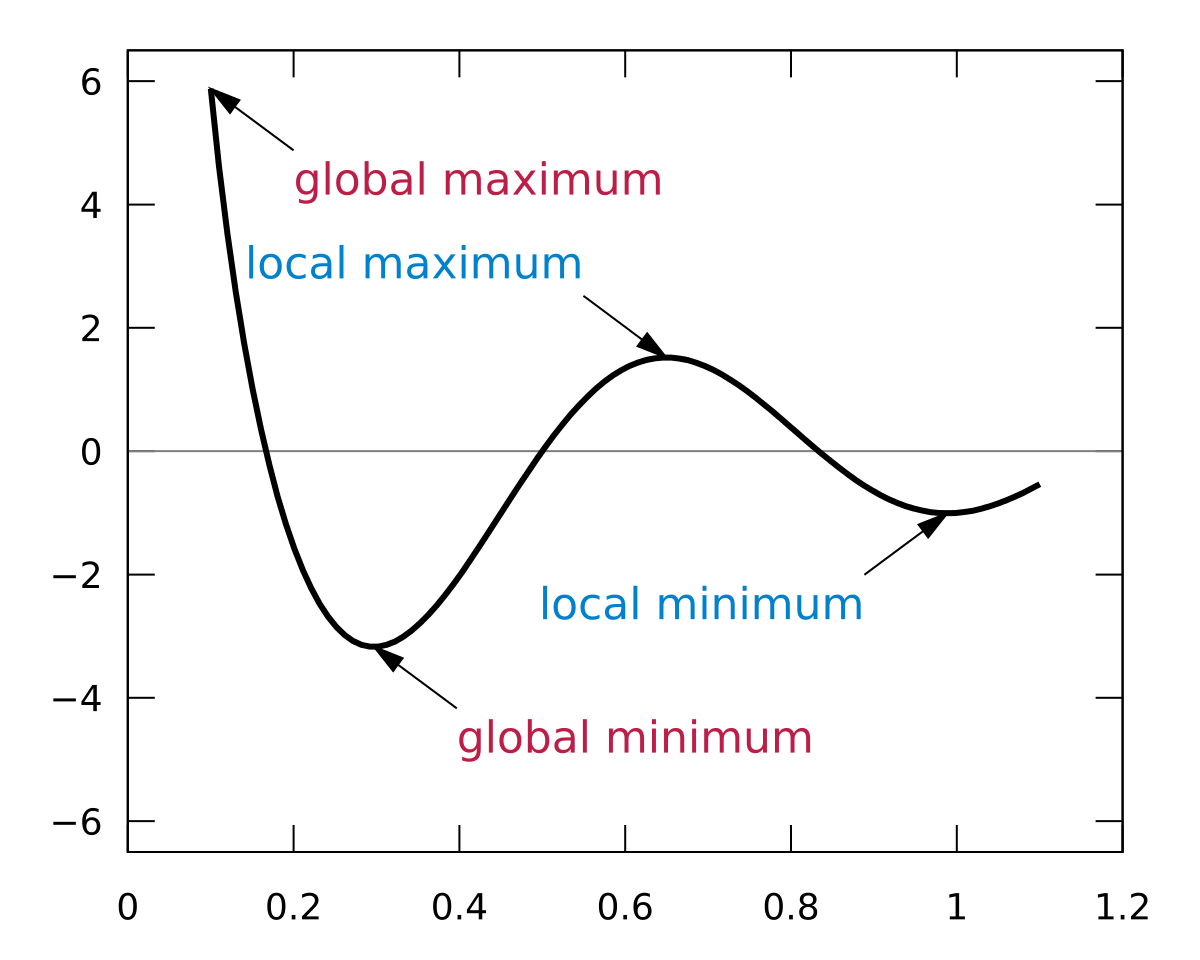
\includegraphics[width=0.5\textwidth]{algebra-pre-calculus/functions/graph7.png}
	\caption{Absolute Maximum and Minimum with Local Maximum and Minimum}
\end{figure}

\subsection{Example}


\begin{align*}
	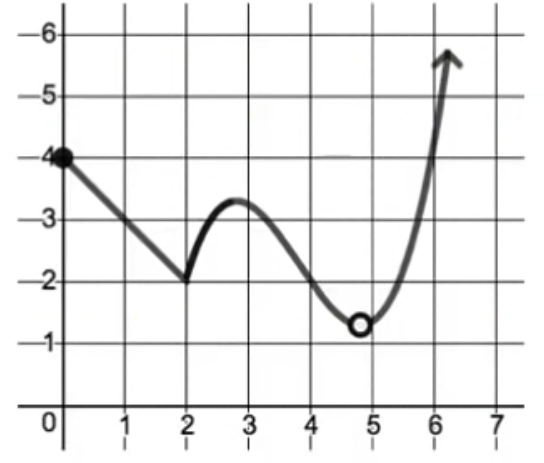
\includegraphics{algebra-pre-calculus/functions/example_graph.png}
\end{align*}

\textbf{Example.} 
\begin{enumerate}
	\item Mark all local maximum and minimum points on the graph. 
	\item Mark all absolute maximum and minimum points on the graph.
	\item What are the local maximum and minimum values?
	\item What are the absolute maximum and minimum values?
\end{enumerate}

\textbf{Solution.} \\
The function has a local maximum point here: $(2.7,-3.3)$ \\
There is a local minimum point here: $(2, 2)$ \\
The point with the drilled out circle means that it is not part of the graph. If it would be then that point would be a local minimum point and an absolute minimum point. \\ 
The point $(0,4)$ by some sources considered to be a local maximum point, However by other sources it doesn't. 
Therefore, we do not have any absolute maximum points, as the arrow indicates that the function goes to infinity. \\
We don't have any absolute minimum points either. \\
Now for talking about the values, we can see that the local maximum value is $-3.3$ and the local minimum value is $2$ which are just the y-values of the points. \\
We do not have any absolute maximum or minimum values.

\subsection{Even and Odd Functions}
\textbf{Definition.} A graph is symmetric with respect to the x-axis if whenever $(x,y)$ is on the graph, then $(x,-y)$(its mirror point) is also on the graph, and it has mirror symmetry across the x-axis as the mirror line. \\
\begin{align*}
	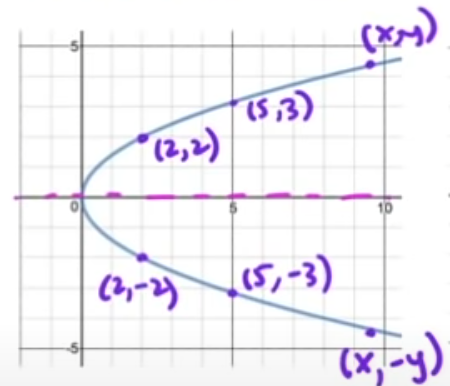
\includegraphics{algebra-pre-calculus/functions/even_odd_graph1.png} \\
\end{align*}

As you can see the graph is symmetric since if we take a point, then the point with the same x-value but with a negative y-value is also on the graph. \\
\textbf{Definition.} A graph is symmetric with respect to the y-axis if whenever $(x,y)$ is on the graph, then $(-x,y)$(its mirror point) is also on the graph, and it has mirror symmetry across the y-axis as the mirror line. \\

\begin{align*}
	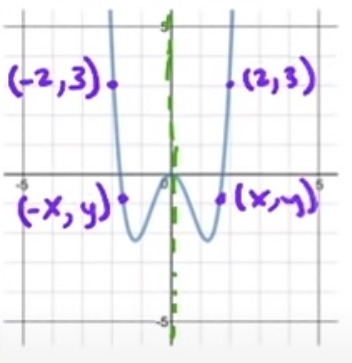
\includegraphics{algebra-pre-calculus/functions/even_odd_graph2.png} \\
\end{align*}

As you can see the graph is symmetric since if we take a point, then the point with the same y-value but with a negative x-value is also on the graph. \\
\textbf{Definition.} A graph is symmetric with respect to the origin if it has 180 degree rotational symmetry around the origin. \\
In other words if we rotate the graph 180 degrees around the origin, then the graph will be the same. \\

\begin{align*}
	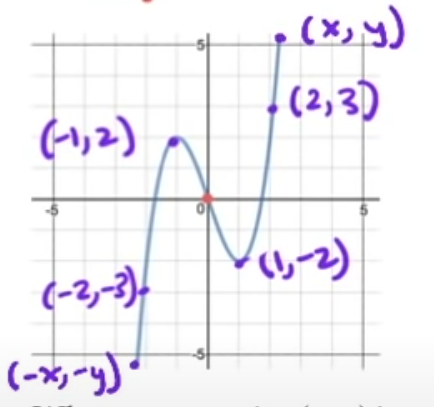
\includegraphics{algebra-pre-calculus/functions/even_odd_graph3.png} \\
\end{align*}
As you can see the origin is the center of the graph and if we rotate the graph 180 degrees around the origin, then the graph will be the same. \\
In terms of the points if we want to find the mirror point of $(x,y)$, then we have to take the negative(opposite, so if it's negative then it should turn to positive) of both the x and y values which is $(-x,-y)$. \\

\subsection{Examples to identify symmetry}

\textbf{Example.} Which graphs are symmetric with respect to the x-axis, the y-axios, the origin or neither? \\

\begin{align*}
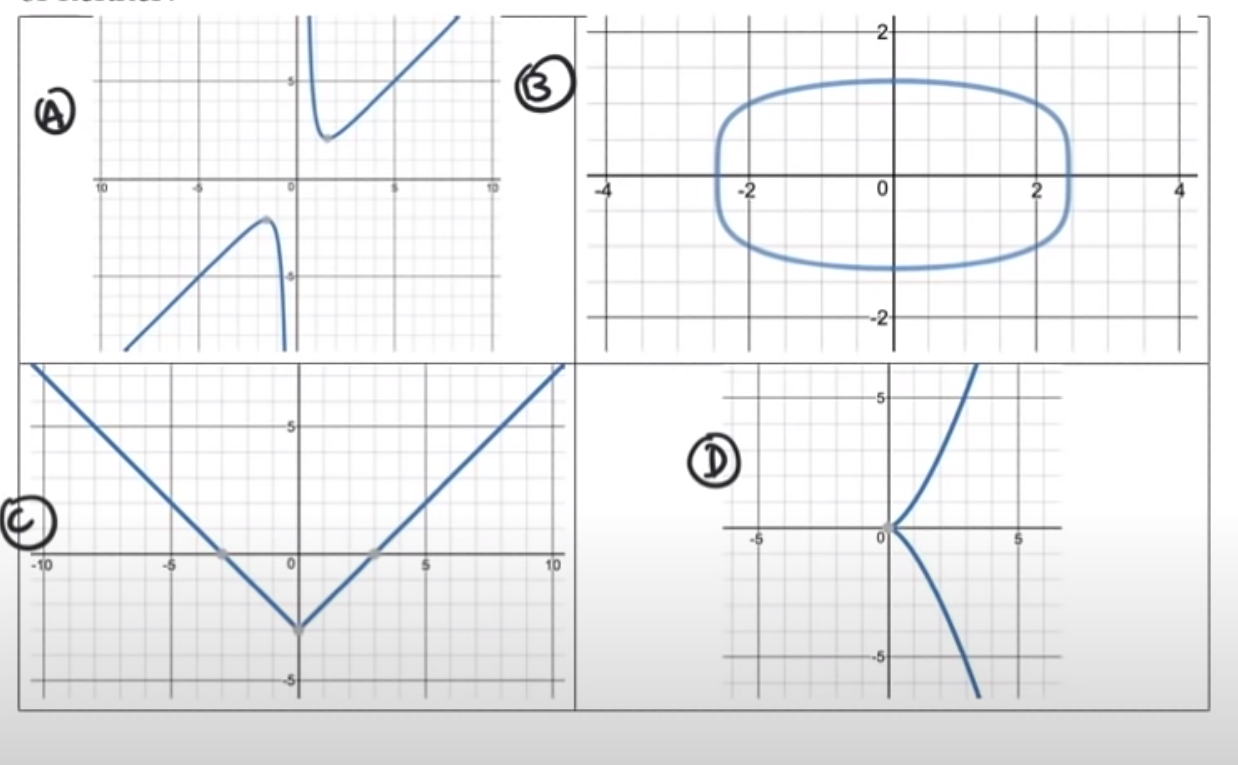
\includegraphics[width=1.2\textwidth]{algebra-pre-calculus/functions/even_odd_example1.png}
\end{align*}

\textbf{Solution.} \\
A. Symmetric with respect to the origin since if we rotate the graph 180 degrees around the origin, then the graph will be the same. \\
B. Symmetric with respect to the y-axis, x-axis, and origin. \\
C. Symmetric with respect to the y-axis. \\
D. Symmetric with respect to the x-axis. \\


\subsection{Even and Odd Functions}

\textbf{Definition.} A function $f(x)$ is even if its graph is symmetric with respect to the y-axis. Meaning that whenever $(x,y)$ is on the graph, then $(-x,y)$(its mirror image) is also on the graph. \\
That is the y-values corresponding to the $x$ and $-x$ are the same. \\
Since $y = f(x)$ we can say that the points are $(x,f(x))$ and $(-x,f(-x))$. \\
In conclusion  we can say that $f(x) = f(-x)$ for all x-values in its domain. Since they are representing the y-values which are the same. 
see here: 
\begin{align*}
	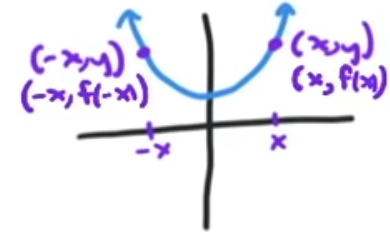
\includegraphics{algebra-pre-calculus/functions/even_odd_example2.png} \\
\end{align*}

\textbf{Example.} $f(x) = x^2+3$ is an even function because... \\
\textbf{Solution.} $f(-x) = (-x)^2+3 = x^2+3 = f(x)$ \\

\textbf{Definition.} A function $f(x)$ is odd if its graph is symmetric with respect to the origin. Meaning that whenever $(x,y)$ is on the graph, then $(-x,-y)$(its mirror image) is also on the graph. \\
The graphs y-value at x and the graphs y-value at -x are the opposites of each other. \\
Since $y = f(x)$ we can say that the points are $(x,f(x))$ and $(-x,-f(-x))$. \\
In conclusion  we can say that $f(-x) = -f(x)$ for all x-values in its domain. This means that the y-values are the opposites of each other. \\
see here:
\begin{align*}
	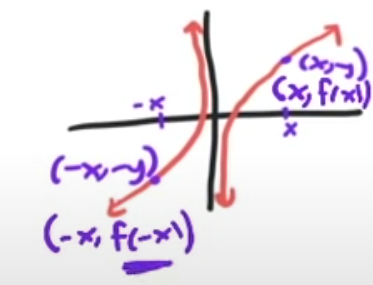
\includegraphics{algebra-pre-calculus/functions/even_odd_example3.png} \\
\end{align*}
\textbf{Example.} $f(x) = 5x-\frac{1}{x}$ is an odd function because... \\
\textbf{Solution.} $f(-x) = 5(-x)-\frac{1}{-x} = -5x+\frac{1}{x} = -(5x-\frac{1}{x}) = -f(x)$ \\

In conclusion we covered that functions that are symmetric with respect to the y-axis are even functions and functions that are symmetric with respect to the origin are odd functions. \\
The reason why we haven't covered functions that are symmetric with respect to the x-axis is because they are neither even nor odd and more importantly they are NOT functions which we will touch on later. \\